%qqqqqqqqqqqqqqqqqqqqqqqqqqqqqqqqqqqqqqqqqqqqqqqqqqqqqqqqqqqqqqqqqqqqqqqqq
%Quote
\begin{savequote}[50mm]
‘‘Equipped with his five senses, man explores the universe around him and 
calls the adventure Science’’
\qauthor{Edwin Hubble}
\end{savequote}
%*************************************************************************




%#########################################################################
\chapter{Preliminaries}
\label{cha:Introduction}


%Reviewed
‘‘What is our place in the cosmos?’’ This is one of the simpler and 
trans\-cendental question that human beings have wondered from ancient 
times; furthermore, this, being powered by our innate curiosity, has led to 
a relatively understandable and structured picture of our Universe. Despite 
of that, this knowledge is very new regarding to our whole history, so the 
astronomy can only be considered as a scientific rigorous discipline since 
the seventeenth century.


%#########################################################################





%*************************************************************************
%Prehistory
\section{Prehistory}
\label{sec:Prehistory}


%Reviewed
Almost in every scientific discipline, a significant theoretical development 
is accompanied by a technical and instrumental improvement. That is why at 
the beginning of the seventeenth century, Johannes Kepler could establish 
his three well-known empirical laws of the planetary movements based upon 
the very precise data of astronomical bodies compiled by Tycho Brahe. This 
event was very remarkable in the history of the astronomy since it was the 
first of many strikes against the well established anthropocentric notion 
of the cosmos. Although Kepler's laws constituted the most crucial test to 
the Nicolaus Copernicus's heliocentric model, it was only until 1685, when 
Isaac Newton formulated the law of universal gravitation (from which can be 
derived all the Kepler's laws), when the astronomers could count with 
enough powerful theoretical tools to start a depth and serious discussion 
about the real nature of our universe on scales bigger than the solar 
system, and thus inaugurating the \textit{sciences of gravity} 
\cite{longair2008}.


%Reviewed
After the establishment of the law of universal gravitation, the next 
significant theo\-retical achievement in this area came in the centuries 
eighteenth and nineteenth with the development of classical mechanics, i.e.
Hamiltonian and Lagrangian formalism, and powerful numerical tools. All
those achievements propelled the study of key topics like the many body 
problem, chaotic phenomenons, etc. Allowing a depth understanding of the 
dynamic of complex gravitational systems, such as planetary systems, star 
clusters, etc. 


%Reviewed
Parallel to the previous theoretical advances, on the observational branch 
was beginning to arise the idea of \textit{island universe}, from which 
would evolve the concept of galaxy. All of this was powered by the 
development of the telescope, furthermore allowing to understand that  
galaxies are just a large collection of stars like our sun. It was also 
very remarkable the pioneer work of William Herschel, who tried to build a
complete map of our galaxy determining distances from the assumption of 
stars with the same intrinsic luminosity and with the inverse square law 
for the intensity decay (see figure \ref{fig:HerschelModel}). 
Although his results were very imprecise due to the incorrect assumption 
on which were based, the importance of his work lies on the recognition of 
some structure (disk-like) for our galaxy. 


%.........................................................................
%Herschel Model of Our Galaxy
\begin{figure}[htbp]
	\centering
	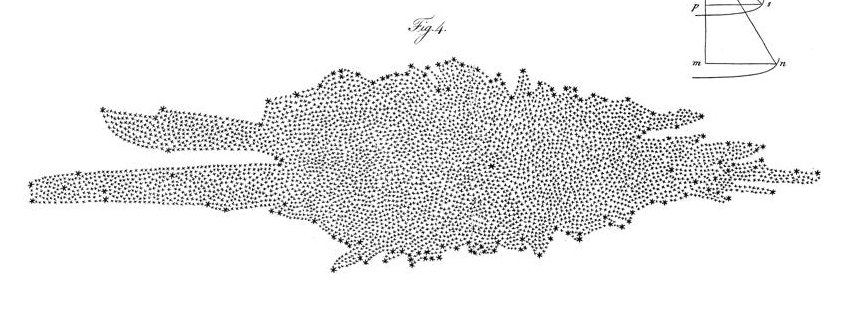
\includegraphics[width=1.0\textwidth]
	{./figures/1_introduction/Herschel_Model.png}
	
	\caption{\small{William Herschel's model for our galaxy based upon a 
	count of stars with the assumption of equal intrinsic luminosity.
	\cite{Herschel1785}.}}
	
	\label{fig:HerschelModel}
\end{figure}
%.........................................................................
\newpage

%Reviewed
Another important observational question, that was emerging among 
scientists by that time, was the existence of \textit{island universes} 
like ours. It was already well-known the existence of extended objects 
that do not fit to the definition of stars or planets, like nebulae, 
planetary disks and galaxies. Even, William Herschel and his son, John 
Herschel, contributed with the realization of a large (for the epoch) 
catalogue of extended bodies known as \textit{Catalogue of Nebulae and 
Clusters of Stars} and a subsequent improved and expanded version finished 
by John Dreyer in 1888, \textit{New General Catalogue of Nebulae and 
Clusters of Stars}, which together with \textit{Index Catalogues} of 1895 
and 1908 constitute a large collection of bodies widely used in current 
astronomy, referred with the abbreviations \textit{NGC} and \textit{IC} 
respectively \cite{longair2008}. Despite of those observational advances, 
the real nature of these objects was a complete mystery, especially if they 
lie within our own galaxy or are completely independent systems. 


%Reviewed
This question remained unsolved until the twentieth century, and together 
with the indetermination of the real size of the universe, were the two 
big issues treated on the well-known \textit{Great Debate}, or also called 
the \textit{Shapley-Curtis Debate}. In this important event in the history 
of astronomy, the astronomers Harlow Shapley and Herber Curtis discussed 
about these topics, giving, respectively, different arguments for and 
against if these objects are within our galaxy and if the Milky Way is our 
whole universe or not \cite{Curtis1921} \cite{Shapley1921}. Despite of 
that, their arguments were not very conclusive and the definitive solution 
to these issues had to wait until 1924, when Edwin Hubble measured the 
distance to Andromeda Galaxy (M31 or NGC 224) and demonstrated 
unquestionably the real extragalactic nature of this object, and in 
following years for other ones \cite{Hubble1926}. This achievement along 
with the observational verification of the expanding universe (also due to 
Hubble) were the beginning of the modern observational cosmology.


%Reviewed
It also happened in the twentieth century a key event for the modern 
sciences of gravity, Albert Einstein formulated his theory of General 
Relativity \cite{Einstein1916}, challenging and changing completely the 
previous conception of space and time and laying the foundation of current 
cosmology picture.


%*************************************************************************




%*************************************************************************
%The current cosmology picture
\section{The Current Cosmology Picture }
\label{sec:TheCurrentCosmologyPicture}


%Reviewed
The theoretical basis on which are based the theory of general relativity
began to arise with the zenith of non-euclidean geometries in the 
nineteenth century and the beginning of twentieth, when it was demonstrated 
that the Euclid's fifth postulate is not needed to build self-consistent 
geometries, thus giving rise to non-planar geometries (see figure 
\ref{fig:NonEuclidean}). In particular, it was highlighted the work of 
Nikolai Lobachevsky, father of non-euclidean geometries, and Bernhard 
Riemman, the founder of the Riemannian geometry.


%.........................................................................
%Herschel Model of Our Galaxy
\begin{figure}[htbp]
	\centering
	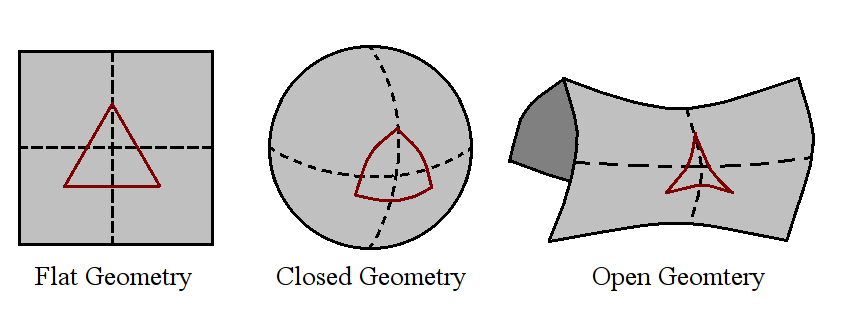
\includegraphics[width=0.9\textwidth]
	{./figures/1_introduction/Non_Euclidean.png}
	
	\caption{\small{Different geometries according to variations on	
	Euclid's fifth postulate.}}
	
	\label{fig:NonEuclidean}
\end{figure}
%.........................................................................


%Reviewed
In spite of these first developments contributed widely to the current 
cosmological paradigm, bringing forward discussions on what kind of 
geometry the universe has, the concepts of space and time were completely 
misunderstood yet, being interpreted as unrelated and absolute entities.
That is why the foundation of the theory of general relativity opened the
door to our whole current understanding.


%Reviewed
Once obtained the equations of metric field of the general relativity, it 
was possible to build global and self-consistent models of the universe.
A first rough attempt was also due to Einstein, who formulated, influenced
by his own belief, a static and closed model of the universe. To achieve it,
he must use the well-known cosmological constant in order to compensate the
expansion/contraction obtained naturally by the theory.


%Reviewed
Few year later, Aleksander Friedmann demonstrated on two articles a 
set of solutions for closed and hyperbolic universes'\ expanding from a
singularity \cite{FriedmanA} \cite{FriedmanB}. These expanding solutions 
were in agreement with the observations made by Hubble for redshift of 
far galaxies. Because of that, the inclusion of the cosmological constant 
for stationary solutions it is historically known and recognized by 
Einstein himself as the biggest blunder of his life. This theoretical 
finding prompted a set of studies on the real nature of the universe in 
the light of those new solutions, like large-scale dynamics, global 
geometry and precise measurements of different cosmological parameters of
those models.


%Reviewed
The next important advance came with the formulation of the Big Bang 
theory by George Gamow. This theory proposes that early stages of 
the universe had been very dense and hot, starting from a singularity and 
reaching the current stage, a constantly cooling and expanding universe. 
All this is in agreement with the Friedmann's solutions. One of the first 
predictions of this theory was the early nucleosynthesis, which is 
responsible of the creation of heavy elements like helium and lithium 
through fusion reactions of primordial hydrogen. Because of the current 
abundances of helium and lithium cannot be given account by the standard
nuclear processes in stars, this was the first of many achievement of the 
Big Bang theory; furthermore the early nucleosynthesis was later 
demonstrated by Ralph Alpher and Robert Herman and it has been 
observationally corroborated very precisely nowadays.

\
%.........................................................................
%Cosmic Background Radiation
\begin{figure}[htbp]
	\centering
	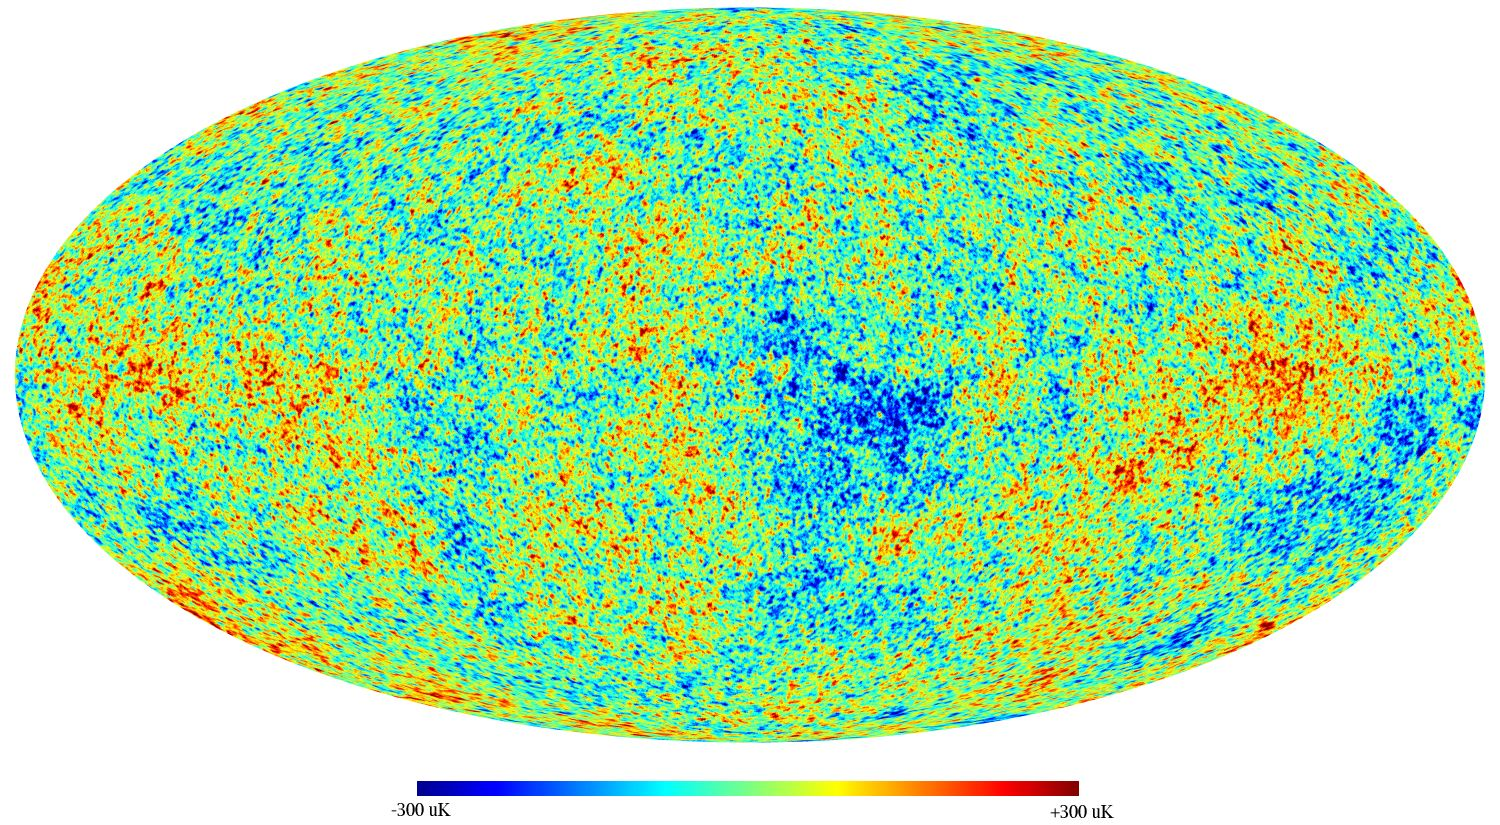
\includegraphics[width=0.8\textwidth]
	{./figures/1_introduction/CMB.png}
	
	\caption{\small{Cosmic background radiation. Taken from 
	\url{http://upload.wikimedia.org/wikipedia/commons/3/3c/Ilc_9yr_moll4096.png}}}
	
	\label{fig:CMB}
\end{figure}
%.........................................................................



The next remarkable prediction of the Big Bang theory was the current 
existence of a residual black-body radiation from the early stages, when,
due to the conditions of high density and temperature, the universe was 
radiation-dominated.


Esto fue corroborado por observacionalmente por Arno Penzias y Robert
Wilson en 1965 con el descubrimiento de la radiación cósmica de microondas
(CBM por su siglas en inglés), donde se midió un espectro de cuerpo negro
de fondo en el universo con una temperatura asociada de $T = 2.725$ K. 
Estas dos predicciones de al teoría del Big Bang han hecho que sea 
adoptado como parte del modelo cosmológico estándar.


Uno de los primeros problemas originados con el descubrimiento de la 
radiación cósmica de fondo es el problema de horizonte. Esto surge debido
la alta isotropía angular medida en el espectro de radiación de fondo (ver 
figura \ref{fig:CMB}), indicando una conexión causal entre regiones tan 
apartadas del universo, que en principio no deberían estarlo. La solución 
al problema fue propuesta por Alan Guth en 1980 y se denomina teoría de 
inflación. En esta se postula una expansión exponencial en el universo 
temprano impulsada por un campo escalar (inflatón). En este periodo de 
expansión se magnificaron las fluctuaciones cuánticas del vacío de todos 
los campos presentes en el universo, produciendo así pequeñas perturbaciones 
en el campo de densidad de las cuales luego evolucionarían las estructuras 
a gran escala de la actualidad. Acorde a esto, la teoría inflacionaria 
también explica satisfactoriamente el problema de pequeñas perturbaciones 
en el universo primigenio, convirtiéndose así en parte del paradigma 
cosmológico actual.


La existencia de la materia oscura fue propuesta desde principios de la 
década de 1930, primero por parte de Jan Oort en 1932 y luego por Fritz
Zwicky en 1933, para dar cuenta de materia no lumínica en galaxias y 
cúmulos galácticos que se manifiesta de forma dinámica. A pesar de esto 
su naturaleza física era completamente desconocida. En 1984 Joel Primack,
George Blumenthal, Sandra Moore y Martin Rees propusieron un modelo de 
materia oscura fría (CDM por sus siglas en inglés), para el cual la 
materia oscura corresponde a un tipo de partícula no relativista que solo
interactua gravitacionalmente y de forma muy débil electromagnéticamente.
Bajo este esquema es posible demostrar que la formación de estructuras a 
gran escala se da de forma jerárquica en un proceso de \textit{top-down},
en el cual las estructuras más pequeñas se forman primero y a partir de 
agrupación de estas se forman las estructuras de gran escala, lo que ha 
sido verificado observacionalmente por surveys de galaxias (ver sección
\ref{sec:CosmologicalObservations}).


En la década de 1990 algunas observaciones cosmológicas comenzaron a 
mostrar una rata de expansión acelerada para el universo, lo que solo 
puede ser explicado (ver subsección \ref{subsec:SimpleSolutionsOfTheUniverse})
con la inclusión de una constante cosmológica en las ecuaciones de campo
de la relatividad general. El término de energía oscura fue acuñado debido 
a que esta constante puede tomarse como una densidad física de energía que
actúa con una presión negativa, impulsando así la rata de expansión del 
universo, a pesar de esto su naturaleza física es completamente incierta.
Mediciones precisas muestran que actualmente el universo está dominado por 
este tipo energía, alcanzando el $70 \%$ del total de materia-energía 
presente en el universo. Eso último completa el paradigma cosmológico 
actual y es denominado modelo estándar $\Lambda$CDM o modelo de 
concordancia.

\
%.........................................................................
%Local Group
\begin{figure}[htbp]
	\centering
	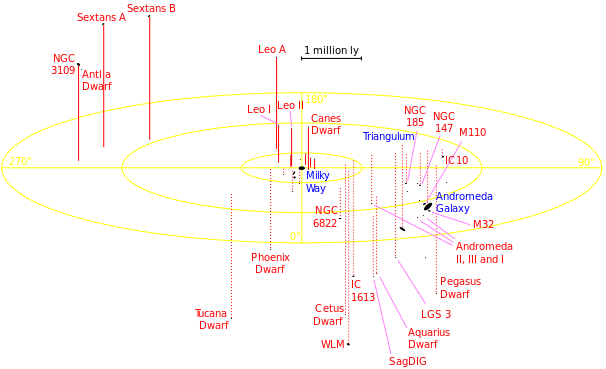
\includegraphics[width=1.0\textwidth]
	{./figures/1_introduction/LocalGroup.png}
	
	\caption{\small{Grupo Local. Tomado de 
	\url{http://commons.wikimedia.org/wiki/File:Local_Group.svg}}}
	
	\label{fig:LocalGroup}
\end{figure}
%.........................................................................


El grupo local es un sistema de aproximadamente 30 galaxias que interactúan
gravitacionalmente entre ellas y evolucionan de forma relativamente aislada
de otras estructuras a gran escala, con la Vía Láctea y Andrómeda como 
miembros más representativos (ver figura \ref{fig:LocalGroup}).


La importancia del grupo local en un contexto cosmológico se debe a que es
la estructura a gran escala más conocida, permitiendo así verificar las 
predicciones del modelo cosmológico estándar. Entre los problemas actuales
en esta línea destacan la sobreabundancia de galaxias satélites para la 
Vía Láctea, la conexión entre los flujos de las nubes de Magallanes y la
galaxia de Andrómeda, fuerzas de marea en el grupo local, la cinemática 
de Andrómeda y la Vía Láctea en un contexto cosmológico \cite{forero2013}
y la influencia del entorno cosmológico en la formación de sistemas como
el grupo local.


%*************************************************************************





%*************************************************************************
%Cosmological observations
\section{Observaciones Cosmológicas}
\label{sec:CosmologicalObservations}
	

El auge generado por la era espacial junto con el gran avance tecnológico
de ins\-trumentos de medida y sensores ha potenciado enormemente las 
investigaciones observacionales en cosmología, permitiendo en conjunto con 
los avances teóricos llegar al paradigma cosmológico actual y contrastar los 
diferentes modelos que han surgido. A continuación se presentan algunos de 
los proyectos observacionales más destacados en cosmología y que son 
ampliamente usados en investigaciones actuales.


	%---------------------------------------------------------------------
	%2DF Galaxy Redshift Survey
	\subsection*{2DF Galaxy Redshift Survey}
	\label{subsec:2DFGRS}
	%---------------------------------------------------------------------
	
	
El 2DF Galaxy Redshift Survey (2DFGRS) o sondeo de corrimiento al rojo en 
un campo de 2 grados\footnote{Página oficial del proyecto 
\url{http://magnum.anu.edu.au/~TDFgg/}.}, es un sondeo del corrimiento al 
rojo de un conjunto de galaxias dentro de una área de $1500$ grados cuadrados 
para zonas cercanas al polo sur y norte galáctico esto para evitar la extinción 
provocada por el disco galáctico. Fue realizado por el telescopio de $3.9$ m 
del observatorio Anglo-Australiano entre 1997 y 2002. Entre los principales 
resultados de este sondeo destaca el establecimiento de la estructura local 
a gran escala en torno al grupo local a partir de medidas fotométricas de 
$382\ 323$ objetos para corrimientos al rojo menores a $z=0.3$, también 
destaca la medida del parámetro de densidad de materia no relativista (
oscura + bariónica) en el modelo cosmológico estándar.

	
	%---------------------------------------------------------------------
	%Sloan Digital Sky Survey
	\subsection*{Sloan Digital Sky Survey}
	\label{subsec:SDSS}
	%---------------------------------------------------------------------


El Sloan Digital Sky Survey (SDSS) o sondeo digital del espacio Sloan, al 
igual que el 2DFGRS es un sondeo en corrimiento al rojo del universo a 
gran escala realizado por el telescopio de $2.5$ m en el observatorio Apache 
Point en Nuevo México desde el año 2000.


%.........................................................................
%SDSS
\begin{figure}[htbp]
	\centering
	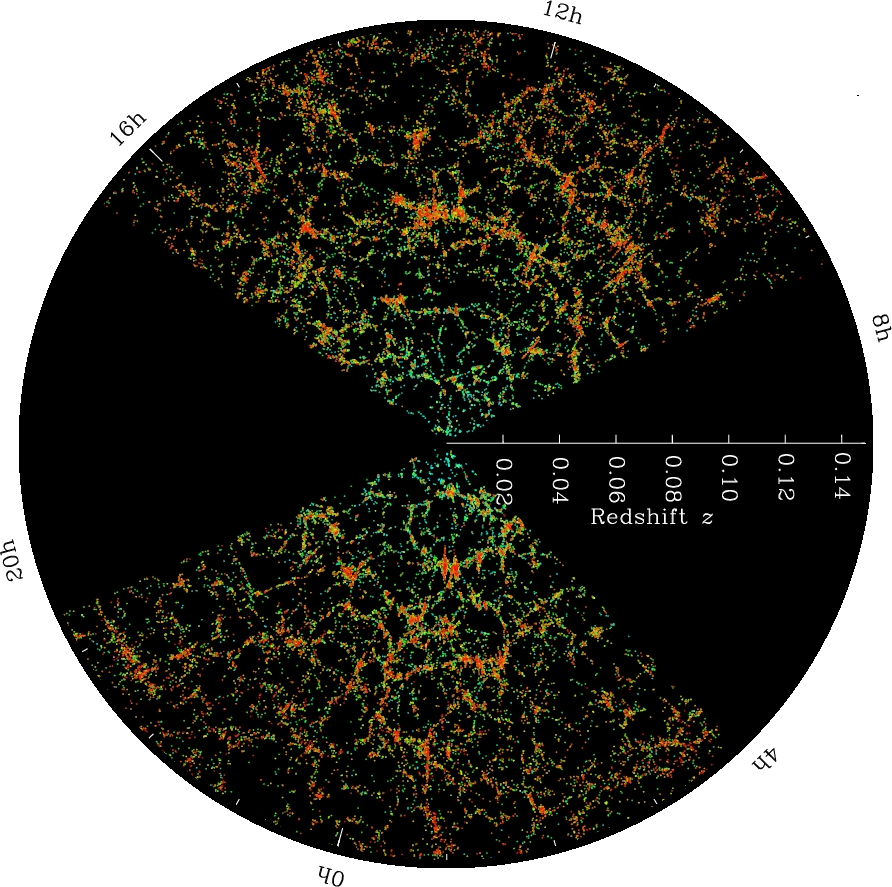
\includegraphics[width=0.6\textwidth]
	{./figures/1_introduction/SDSS.png}
	
	\caption{\small{Mapa del universo a gran escala de acuerdo al Sloan 
	Digital Sky Survey. Tomado de la página oficial del proyecto 
	\url{http://www.sdss.org/}}}
	
	\label{fig:SDSS}
\end{figure}
%.........................................................................


El sondeo cubre una zona significativamente mayor que el 2DFGRS, 
aproxi\-madamente $7500$ grados cuadrados y ha catalogado alrededor de 
$2$ millones de objetos, permitiendo construir un mapa a gran escala del 
universo y percibir por primera vez la estructura de la red cósmica 
(ver figura \ref{fig:SDSS}).
	
	
	%---------------------------------------------------------------------
	%WMAP
	\subsection*{WMAP}
	\label{subsec:WMAP}
	%---------------------------------------------------------------------


La Wilkinson Microwave Anisotropy Probe (WMAP), es una sonsa espacial de 
la NASA lanzada en 2001 y ubicada en el punto de Lagrange L2. Su principal 
objetivo es medir con muy alta precisión los pequeños contrastes de 
temperatura y la polarización de la radiación cósmica de fondo (ver figura 
\ref{fig:CMB}). Aproximadamente cada 2 años la NASA libera los resultados
acumulados obtenidos, referidos como WMAP1, WMAP3, WMAP5, WMAP7 y 
finalmente en el 2012 el WMAP9. Los resultados obtenidos por el WMAP han 
sido hasta el momento la prueba más fehaciente del modelo cosmológico 
estándar $\Lambda$CDM. En especial destacan la medida precisa de la edad del
universo, los diferentes parámetros de densidad, la constante de Hubble, 
la determinación de la geometría global del universo (plana) y la 
confirmación del modelo inflacionario.

\
%.........................................................................
%Cosmological Parameter of WMAP7
\begin{table}[htbp]
\begin{small}
\centering
\begin{tabular}{|c|c|c|c|} \hline
\cellc{\textbf{Parameter}}		&
\cellc{\textbf{Notation}}		&  
\cellc{\textbf{Value}}			& 
\cellc{\textbf{Unit}}					\\ \hline


Age of universe 			&	$t_0$			&	$13.75 \pm 0.13$	&	Ga 			\\ \hline

Hubble's constant			&	$H_0$			&	$71.0 \pm 2.5$		&   km/(Mpc s)	\\ \hline

Hubble's parameter			&	$h$				&	$0.71 \pm 0.025$	&   --			\\ \hline

Barion density		&	$\Omega_b$		&	$0.0449\pm 0.0027$	&	--			\\ \hline

Dark matter & & & \\
density				&	$\Omega_c$		&	$0.222 \pm 0.026$	&	--			\\ \hline

Dark energy & & & \\
density				&	$\Omega_\Lambda$&	$0.734 \pm 0.029$	&	--			\\ \hline

Radiation & & & \\
density					&	$\Omega_r$		&$8.24 \times 10^{-5}$	&	--			\\ \hline

Amplitude of & & & \\
Fluctuations at $8h^{-1}$ Mpc&	$\sigma^2_8$	&	$0.801 \pm 0.030$	&	--			\\ \hline

Spectral index			&	$n_s$			&	$0.963 \pm 0.014$	&	--			\\ \hline
Reionization & & & \\
optic depth 			&	$\tau$			&	$0.088 \pm 0.015$	&	--			\\ \hline
				
Total density of & & & \\
the Universe	&	$\Omega_0$		&	$1.080\ \mbox{\scriptsize{$+0.093$}}/ 
										\mbox{\scriptsize{$-0.071$}} $&	--				\\ \hline
\end{tabular}
\caption{WMAP7 cosmological parameters \cite{WMAP7}.}
\label{tab:CosmologicalParameters}
\end{small}
\end{table}
%.........................................................................


En la tabla \ref{tab:CosmologicalParameters} se tabulan los resultados 
del WMAP7 \cite{WMAP7}, los cuales son ampliamente usados en los siguientes 
capítulos y en especial las diferentes simulaciones cosmológicas presentadas en
los capítulos \ref{cha:N-BodySimulations} y \ref{cha:Results} están basadas
en estos.


%*************************************************************************